% based on a template made by the university of cologne
% http://www.mi.uni-koeln.de/wp-MIEDV/wp-content/uploads/2016/07/LaTeX-Vorlage.zip - 2023-11-02
\documentclass[12pt,a4paper]{scrartcl}

\addtokomafont{sectioning}{\rmfamily}
%\usepackage[ngerman]{babel}% deutsches Sprachpaket wird geladen
\usepackage[T1]{fontenc} % westeuropäische Codierung wird verlangt
\usepackage[utf8]{inputenc}% Umlaute werden erlaubt
\usepackage[usenames]{color} % Erlaubt die Benutzung der namen im Farbpaket und deren Änderung
\usepackage{amsmath} % Erweiterung für den Mathe-Satz
\usepackage{amssymb} % alle Zeichen aus msam und msmb werden dargestellt
\usepackage{graphicx} % Graphiken und Bilder können eingebunden werden
%\usepackage{multirow} % erlaubt in einer Spalte einer Tabelle die Felder in mehreren Zeilen zusammenzufassen
\usepackage{enumerate} % erlaubt Nummerierungen
\usepackage{url} % Dient zur Auszeichnung von URLs; setzt die Adresse in Schreibmaschinenschrift.
\usepackage[center]{caption}  % Bildunterschrift wird zentriert
%\usepackage{subfigure} % mehrere Bilder können in einer fugure-Umgebung verwendet werden
%\usepackage{longtable} % Diese Umgebung ist ähnlich definiert wie die tabular-Umgebung, erlaubt jedoch mehrseitige Tabellen.
%\usepackage{paralist} % Modifikation der bereits bestehenden Listenumgebungen
\usepackage{lmodern}% Für die Schrift
\usepackage[hidelinks]{hyperref} % Links und Verweise werden innerhalb von PDF Dokumenten erzeugt
%\usepackage{wrapfig} % Das Paket ermöglicht es von Schrift umflossene Bilder und Tabellen einzufügen.
\usepackage{latexsym} % LaTeX-Symbole werden geladen
\usepackage{tikz} % Erlaubt es mit tikz zu zeichnen
\usepackage{tabularx} % Erlaubt Tabellen
\usepackage{algorithm} % Erlaubt Pseudocode
\usepackage{color} % Farbpaket wird geladen
%\usepackage{stmaryrd} % St Mary Road Symbole werden geladen

\numberwithin{equation}{section} % Nummerierungen der Gleichungen, die durch equation erstellt werden, sind gebunden an die section
\newcommand{\HRule}{\rule{\linewidth}{0.7mm}}
\newcommand{\pu}[1]{\ensuremath{\mathrm{#1}}}

% disable commands
\renewcommand{\[}{} % math block start
\renewcommand{\]}{\noindent} % math block end
\newcommand{\tightlist}{} % created in enumerations

\hypersetup{
  pdftitle={B 2.4},
  pdfcreator={LaTeX via pandoc}}

\begin{document}
\begin{titlepage}
	\pagestyle{empty}

	\begin{center}

	\textsc{\LARGE Universität zu Köln }\\ [0.4cm]
	\textsc{Mathematisch-Naturwissenschaftliche Fakultät} \\[1.5cm]

	\includegraphics[width=0.45\textwidth]{uni}\\[1.5cm]  % Uni-Logo wird geladen

	\textsc{\Large Praktikum~B}\\[2mm]
	\textsc{}\\[10mm]
	\HRule \\[0.4cm]

		{	\Huge \bfseries B 2.4}\\[0.4cm]
			{	\huge \bfseries Magnetisierung eines Ferrits}\\[0.3cm]
	
	\HRule \\[3cm]

			\textsc{\Large Catherine Tran } \\[3pt]
		\textsc{\Large Carlo Kleefisch } \\[3pt]
		\textsc{\Large Oliver Filla } \\[3pt]
		
% 	\begin{center}
% 	\textsc{\Large Catherine~Tran } \\[3pt]
% 	\textsc{\Large Carlo~Kleefisch } \\[3pt]
% 	\textsc{\Large Oliver~Filla } \\[3pt]
% 	\end{center}
	\end{center}
\end{titlepage}

\newpage
\tableofcontents
\newpage

\hypertarget{motivation}{%
\section{Motivation}\label{motivation}}

In diesem Versuch werden Ordnungsphänomene von ferromagnetischen
Materialien behandelt. Hierzu werden die Magnetisierungskurven an zwei
verschiedenen Aufbauten aufgenommen. Deren zentraler Bestandteil ein
Ringkern aus einem Ferrit-Werkstoff ist.

Anhand dieser Kurven lassen sich zahlreiche Eigenschaften dieses
Ringkerns untersuchen, wie zum Beispiel die Suszeptibilität, das
Temperatur- und das Entmagnetisierungsverhalten.

Mithilfe dieses Versuchs kann ein Einblick in Phänomene des Magnetismus
erlangt werden. Dessen Wirkung beschäftigt Menschen schon seit hunderten
von Jahren und welcher Grundlage für zahlreiche technische Anwendungen
ist.

\hypertarget{theoretische-grundlagen}{%
\section{Theoretische Grundlagen}\label{theoretische-grundlagen}}

\hypertarget{grundlagen-des-magnetismus}{%
\subsection{Grundlagen des
Magnetismus}\label{grundlagen-des-magnetismus}}

Das Phänomen des Magnetismus kann nicht klassisch erklärt werden,
sondern muss durch die Quantenmechanik beschrieben werden. Sie befasst
sich mit Strömen, was sie qualitativ von der Elektrostatik
unterscheidet.

Die wichtigsten Größen sind die \emph{Flussdichte} \(\vec B\), die
\emph{Magnetisierung} \(\vec M\) und die \emph{Feldstärke} \(\vec H\).
Diese werden durch die \emph{Feldkonstante}
\(\mu_0=4\pi\cdot\pu{10^{-7}\frac{Vs}{Am}}\) bzw. die
\emph{Permeabilität} \(\mu\) miteinander in Verbindung gebracht. Die
Permeabilität beschreibt die Durchlässigkeit für magnetische Felder.
\([2]\)

\[
\begin{eqnarray}
    \vec B
        &=& \mu_0 \cdot \left(\vec H + \vec M\right) \label{M1} \\
        &=& \mu \cdot \vec H
\end{eqnarray}
\]

Die \emph{Suszeptibilität} \(\chi\) ist eine dimensionslose Größe,
welche die Magnetisierbarkeit von Materie beschreibt. Sie beschreibt die
Änderung der Magnetisierung \(\vec M\) durch die Änderung der Feldstärke
\(\vec H\).

\[
\begin{eqnarray}
    \chi &=& \frac{\mathrm dM}{\mathrm dH} \label{Chi}
\end{eqnarray}
\]

Das magnetische Dipolmoment \(\vec \mu\) tritt auf, wenn elektrische
Ladungen sich auf Kreisbahnen bewegen. Es lässt sich über das auf einen
magnetischen Dipol wirkende Drehmoment \(\vec \tau\) in einem Magnetfeld
\(\vec B\) definieren.

Für eine ebene Leiterschleife ist es folgendermaßen beschrieben. \([2]\)
Die Dichte des magnetischen Momentes wird durch die Magnetisierung
beschrieben.

\[
\begin{eqnarray}
    \vec \tau &=& \vec \mu \times \vec B \\
    \vec M &=& \frac{\vec \mu}{V}
\end{eqnarray}
\]

Das Magnetfeld im Inneren einer Spule kann durch den Strom \(I\), die
Windungszahl \(n\) und die Länge der Spule \(l\) beschrieben werden.
Dabei ist \(\vec e_z\) der Einheitsvektor längs der Spule, d.h.
senkrecht zur Querschnittsfläche derselben. \([2]\)

\[
\begin{eqnarray}
    \vec H &=& \frac{In}{l} \vec e_z
\end{eqnarray}
\]

Für eine einzelne Leiterschleife ist das Magnetfeld dagegen durch die
eingeschlossene Fläche \(A\) zu beschreiben, sowie durch den
Einheitsvektor \(\vec e_A\) senkrecht zu \(A\).

\[
\begin{eqnarray}
    \vec H &=& IA \vec e_A
\end{eqnarray}
\]

\hypertarget{magnetismus-ohne-ordnungsphuxe4nomene}{%
\subsection{Magnetismus ohne
Ordnungsphänomene}\label{magnetismus-ohne-ordnungsphuxe4nomene}}

\hypertarget{bahnmagnetismus-und-spinmagnetismus}{%
\subsubsection{Bahnmagnetismus und
Spinmagnetismus}\label{bahnmagnetismus-und-spinmagnetismus}}

Der Bahnmagnetismus beschreibt das magnetische Moment \(\vec m_l\) eines
Teilchens aufgrund seiner Bahnbewegung durch den Bahndrehimpuls. Analog
gibt es Spinmagnetismus, dieser beschreibt das magnetische Moment eines
Teilchens aufgrund seines Spins.

Besitzt ein Teilchen sowohl ein Bahndrehimpuls \(\vec L\) als auch einen
Spin \(\vec S\), so lässt sich das gesamte magnetische Moment
\(\vec{m}\) dieses Teilchens ausdrücken als:

\[
\begin{eqnarray}
    \vec m &=& \vec m_l + \vec m_s
\end{eqnarray}
\]

Alternativ sind das magnetische Moment \(\vec{m}\) und der
Gesamtdrehimpuls \(\vec{J}\) über das gyromagnetische Verhältnis
\(\gamma\) miteinander verknüpft.

\hypertarget{gyromagnetisches-verhuxe4ltnis}{%
\subsubsection{gyromagnetisches
Verhältnis}\label{gyromagnetisches-verhuxe4ltnis}}

Das magnetische Moment \(\vec{m}\) und der Gesamtdrehimpuls \(\vec{J}\)
sind über das gyromagnetische Verhältnis \(\gamma\) miteinander
verknüpft. \([6]\) Dabei wird \(\gamma\) durch das Planck'sche
Wirkungsquantum \(\hbar\), das Bohr'sche Magneton \(\mu_{B}\) und den
Lande-Faktor \(g\) bestimmt.

\[
\begin{eqnarray}
    \gamma &=& \frac{g\mu_B}{\hbar} \\
    \vec{m} &=& \gamma \vec{J}
\end{eqnarray}
\]

Besitzt ein Teilchen sowohl ein Bahndrehimpuls \(\vec L\) als auch einen
Spin \(\vec S\), so lässt sich das gesamte magnetische Moment
\(\vec{m}\) durch Bahnmagnetismus und Spinmagnetismus darstellen.

\[
\begin{eqnarray}
    \vec m &=& \vec m_l + \vec m_s
\end{eqnarray}
\]

\%\%{[}{[}@Gross2012Festkörper\textbar Gross, Festkörperphysik{]}{]}, S.
761\%\%

\hypertarget{lande-faktor}{%
\subsubsection{Lande-Faktor}\label{lande-faktor}}

Der Lande-Faktor \(g\) bestimmt das gyromagnetische Verhältnis
\(\gamma\).

Für ein Elektron ist der Lande-Faktor \(g\) durch den Gesamtdrehimpuls
\(J\), den Spin \(S\) und den Bahndrehimpuls \(L\) bestimmt. \([6]\) Im
Falle reinen Spinmagnetismus gilt \(g_{s} \approx 2\), ebenso bei reinem
Bahnmagnetismus.

\[
\begin{eqnarray}
    g &=& 1 + \frac{J(J+1) + S(S+1) + L(L+1)}{2J(J+1)}
\end{eqnarray}
\]

Die einzelnen Terme, z.B. \(J(J+1)\), sind proportional zu dem
Erwartungswert der quadrierten Drehimpulsoperatoren, in diesem Beispiel
\(\hat J^2\).

\%\%{[}{[}@Gross2012Festkörper\textbar Gross, Festkörperphysik{]}{]}, S.
1044\%\%

\hypertarget{bohrsches-magneton}{%
\subsubsection{Bohr'sches Magneton}\label{bohrsches-magneton}}

Das Bohr'sche Magneton \(\mu_B\) beschreibt das magnetische Moment, das
ein Elektron durch seine Rotation um den Atomkern erzeugt. Seine Einheit
ist Energie pro Tesla.

\[
\begin{eqnarray}
    \mu_B &=& \frac{e\hbar}{2m_e} \\
    \mu_B &\approx& \pu{5.788 \cdot 10^{-5} \frac{eV}{T}} \\
    \mu_B &\approx& \pu{9.274 \cdot 10^{-24} \frac{J}{T}}
\end{eqnarray}
\]

\hypertarget{diamagnetismus}{%
\subsubsection{Diamagnetismus}\label{diamagnetismus}}

Ein diamagnetischer Festkörper besitzt keine inneren magnetischen
Momente. Durch ein äußeres Magnetfeld werden aber magnetische Momente im
Festkörper induziert. Diese sind aufgrund der Lenz'schen Regel dem
induzierenden Magnetfeld entgegengesetzt, weshalb die magnetische
Suszeptibilität von diamagnetischen Festkörpern \(\mu_\mathrm{dia}\)
negativ ist.

Für Isolatoren ist \(\mu_\mathrm{dia}\) außerdem von der Temperatur des
Isolators unabhängig.

Perfekter Diamagnetismus ist bei Supraleitern zu finden. Diese weisen
eine magnetische Suszeptibilität von \(\chi_\mathrm{supra} = -1\) auf.

Deshalb wird sich ein beweglicher Diamagnet in einem inhomogenen
Magnetfeld aus diesem herausbewegen, was einen Unterschied zu
Paramagneten darstellt.

Ein diamagnetischer Festkörper besitzt keine inneren magnetischen
Momente. Durch ein äußeres Magnetfeld werden aber magnetische Momente im
Festkörper induziert. Diese sind aufgrund der Lenz'schen Regel dem
induzierenden Magnetfeld entgegengesetzt, weshalb die magnetische
Suszeptibilität von diamagnetischen Festkörpern \(\mu_\mathrm{dia}\)
negativ ist. \([6]\)

Für Isolatoren ist \(\mu_\mathrm{dia}\) außerdem unabhängig von der
Temperatur des Isolators. \([6]\)

Perfekter Diamagnetismus ist bei Supraleitern zu finden. Diese weisen
eine magnetische Suszeptibilität von \(\chi_\mathrm{supra} = -1\) auf.

\%\%{[}{[}@Gross2012Festkörper\textbar Gross, Festkörperphysik{]}{]}, S.
671\%\% \%\%{[}{[}@Gross2012Festkörper\textbar Gross,
Festkörperphysik{]}{]}, S. 679\%\%

\hypertarget{paramagnetismus}{%
\subsubsection{Paramagnetismus}\label{paramagnetismus}}

In einem paramagnetischen Festkörper liegen innere magnetische
Dipolmomente vor, welche z.B. durch Spin und Bahndrehimpuls der
Elektronen herrühren. Diese wechselwirken allerdings nicht miteinander,
wodurch sie nur in einem äußeren Magnetfeld in Richtung des Feldes
ausgerichtet werden. Die magnetische Suszeptibilität
\(\chi_\mathrm{para}\) eines paramagnetischen Festkörpers~ist daher
positiv.

\hypertarget{langevin-paramagnetismus}{%
\paragraph{Langevin-Paramagnetismus}\label{langevin-paramagnetismus}}

Der Langevin-Paramagnetismus liefert Beschreibungen für paramagnetische
Isolatoren. Die magnetische Suszeptibilität \(\chi_\mathrm{langevin}\)
dieser ist durch das Curie-Gesetz durch die Curie-Konstante \(C\) und
die Temperatur \(T\) beschrieben. \([6]\)

\[
\begin{eqnarray}
    \chi_\mathrm{langevin} &=& \frac{C}{T}
\end{eqnarray}
\]

\%\%{[}{[}@Gross2012Festkörper\textbar Gross, Festkörperphysik{]}{]}, S.
688\%\%

\hypertarget{pauli-paramagnetismus}{%
\paragraph{Pauli-Paramagnetismus}\label{pauli-paramagnetismus}}

Der Pauli-Paramagnetismus beschreibt die Eigenschaften von
paramagnetischen Metallen. Die magnetische Suszeptibilität
\(\chi_\mathrm{pauli}\) eines solchen Metalle ist konstant. \([6]\)

\[
\begin{eqnarray}
    \chi_\mathrm{pauli} &=& \mathrm{const}
\end{eqnarray}
\]

Hier tritt keine Temperaturabhängigkeit mehr auf, da aufgrund der
Fermi-Statistik nur grob \(\frac{T}{T_F}\) Elektronen in einem
Energieintervall um die Fermi-Energie ihre Energie ändern können, wobei
\(T_{f}\) die Fermi-Temperatur ist. Dadurch stellt sich ein
temperaturunabhängiger Beitrag
\(\frac{C}{T} \frac{T}{T_F} = \frac{C}{T_F}\) ein. \([6]\)

Der Pauli-Paramagnetismus ist deutlich schwächer als der
Langevin-Paramagnetismus.

\[
\begin{eqnarray}
    \frac{\chi_\mathrm{pauli}}{\chi_\mathrm{langevin}}
        &\propto& \frac{T}{T_F} \ll 1
\end{eqnarray}
\]

\%\%{[}{[}@Gross2012Festkörper\textbar Gross, Festkörperphysik{]}{]}, S.
695-698\%\%

\hypertarget{magnetismus-mit-ordnungsphuxe4nomen}{%
\subsection{Magnetismus mit
Ordnungsphänomen}\label{magnetismus-mit-ordnungsphuxe4nomen}}

\hypertarget{magnetische-ordnung}{%
\subsubsection{magnetische Ordnung}\label{magnetische-ordnung}}

Die magnetische Ordnung wird durch die Austauschwechselwirkung
verursacht. Diese beruht auf dem Pauli-Prinzip.

\hypertarget{magnetische-anisotropie}{%
\subsubsection{magnetische Anisotropie}\label{magnetische-anisotropie}}

Anisotropie ist die Eigenschaft eines Material, die von der Ausrichtung
der magnetischen Drehmomenten abhängt. Dabei bezeichnet man die
energetisch günstigere Ausrichtung als \emph{Achse leichter
Magnetisierung}. Die Kristallstruktur bestimmt über die Art der
Anisotropie. Man unterscheidet zwischen Formanisotropie,
Spannungsanisotropie und Kristallanisotropie.

Im Allgemeinen ist Anisotropiedie Richtungsabhängigkeit einer
Eigenschaft oder eines Vorgangs.

\hypertarget{ferromagnetismus}{%
\subsubsection{Ferromagnetismus}\label{ferromagnetismus}}

Bei Ferromagnetismus richten sich die magnetische Momente parallel
zueinander aus. Im \emph{ferrimagnetischen} Material dagegen sind die
Momente abwechselnd antiparallel zueinander ausgerichtet, dennoch heben
sich die Beträge sich nicht auf wie in einem
\emph{antiferromagnetischen} Material.

\hypertarget{weiuxdfsche-bezirke}{%
\subsubsection{Weiß'sche Bezirke}\label{weiuxdfsche-bezirke}}

Weiß'sche Bezirke sind Bereiche mit gleichartige
Magnetisierungsausrichrung. Der Grenzbereich zwischen zwei Weißschen
Bezirke nennt man \emph{Bloch-Wand}. Auch wenn kein äußeres Magnetfeld
angelegt ist, existieren vereinzelte Bereiche mit parallelen Spins, die
man \emph{Domänen} nennt.

Legt man nun ein Magnetfeld an, verschmelzen kleine Domänen zu größeren
und die Magnetisierung der Stoffes ist messbar. Bei kleiner Feldstärke
findet reversible \emph{Wandverschiebungen} statt, schaltet man die
Feldstärke hoch finden sogenannte ``\emph{Barkhausen-Sprünge}'' statt.
Hierbei ändert sich die Ausrichtung alle magnetischen Momente ganzer
Weiß'scher Bezirke schlagartig, so dass es zu einer deutlichen Änderung
in der Magnetisierungskurve kommt.

Kurz vor der Sättigung finden \emph{Rotationsprozesse} statt, wo dann
alle magnetische Momente in Richtung des äußeren Feldes zeigen.

\hypertarget{hysteresekurve}{%
\subsubsection{Hysteresekurve}\label{hysteresekurve}}

Die Hysteresekurve beschreibt das Verhalten eines Materials im äußeren
Magnetfeld.

Die Kurve startet im Ursprung und steigt (durch
\emph{Wandverschiebungen}) leicht an, dreht man das Feld auf wird die
Kurve wegen der \emph{Barkhausen-Sprünge} steiler. Bei größer werdenden
Feldstärken verläuft sie durch die Rotation wieder flacher zu. Dann
findet die \emph{Sättigung} statt, wo die maximale Magnetisierung
erreicht ist. Diese Kurve bezeichnet man als \emph{Neukurve}.

Entfernt man das Magnetfeld bzw. schaltet man es ab, sinkt die
Magnetisierung nicht automatisch auf null, sondern eine
Restmagnetisierung bleibt übrig, sogenanntes \emph{Remanenz}.

Sollt auch diese verschwinden, muss man ein negatives Feld anlegen und
die \emph{Koerzitivfeldstärke} erreichen, der Stoff ist dann vollständig
entmagnetisiert. Wird die Feldstärke weiter erhöht, magnetisiert der
Stoff in die entgegengesetzte Richtung, bis die Sättigung wieder
auftritt.

Die \emph{Kommutierungskurve} ist die Verbindungskurve der
Hystereseschleifen-Umkehrpunkte. Die Fläche, die die Hysteresekurve
umschließt, entspricht dem Energiegehalt, das erbracht werden muss,
messbar als Wärme.

Anhand der Hysterese kann man erkennen ob eine Probe weichmagnetisch
oder hartmagnetisch ist. \emph{Weichmagnetische} Materialien haben eine
kleine Koerzitivfeldstärke und eine hohe Sättigungsmagnetisierung, sie
sind also leicht zu magnetisieren. Man verwendet diese oft für
Transformatoren und Sensoren.

\emph{Hartmagnetische} Materialien dagegen haben eine große
Koerzitivfeldstärke und einen niedrigen Sättigungspunkt. Sie sind schwer
zu magnetisieren daher baut man daraus oft Dauermagnete.

\hypertarget{temperaturabhuxe4ngigkeit}{%
\subsubsection{Temperaturabhängigkeit}\label{temperaturabhuxe4ngigkeit}}

Magnetische Eigenschaften hängen von der Temperatur ab. Steigt diese,
dann nimmt die Permeabilität ab, also die Ordnung der magnetische
Momente. Durch Erhöhung der Temperatur fügt man dem System Energie zu
und die Austauschwechselwirkung wird dadurch schwächer, bis sie
irgendwann komplett überwunden wird. Dieser Punkt nennt man
\emph{Curie-Temperatur}, nur unter diese ist ein ferromagnetischer Stoff
einsetzbar. Ab der Curie-Temperatur zeigt der Stoff paramagnetische
Verhalten.

\hypertarget{phasenuxfcberguxe4nge}{%
\subsubsection{Phasenübergänge}\label{phasenuxfcberguxe4nge}}

\emph{Ordnungsparameter} beschreibt den Zustand eines System beim
\emph{Phasenübergang}.

Bei Ferromagneten ist der Parameter die Magnetisierung. Beträgt der
Parameter Null, so ist das System völlig ungeordnet. Verläuft ein
Phasenübergang sprunghaft (z.B. vom Wasser zu Eis), klassifiziert man
ihn als \emph{Übergang 1. Ordnung}. Ist der Verlauf kontinuierlich (z.B.
von ferromagnetisch zu paramagnetisch) spricht man von einem
\emph{Übergang 2. Ordnung}.

Hierbei sind sprunghaft und kontinuierlich wie folgt definiert. Die 1.
partielle Ableitung der Enthalpie \(G(T,p)\) nach der Temperatur \(T\)
ist unstetig bzw. stetig.

\emph{Latente Wärme} ist die Wärme, die dazu führt, dass ein Stoff
seinen Aggregatzustand ändert, sie führt deshalb nicht zu einer
Temperaturerhöhung.

\hypertarget{entmagnetisierung}{%
\subsection{Entmagnetisierung}\label{entmagnetisierung}}

Laufen die Feldlinien eines äußeren magnetischen Feldes durch die
Flächen eines Kristalls, so induzieren sie magnetische Dipolmomente im
Kristall. Diesen kann man einen magnetischen Nordpol und einen
magnetischen Südpol zuweisen.

Nach der Lenz'schen Regel wirkt das auf diese Weise induzierte
Magnetfeld dem äußeren Feld entgegen. Dadurch wird das äußere Feld
abgeschwächt, daher nennt man das induzierte Feld auch
\emph{Entmagnetisierungsfeld}.

\hypertarget{entmagnetisierungsfaktor}{%
\subsubsection{Entmagnetisierungsfaktor}\label{entmagnetisierungsfaktor}}

Um einen Stoff mit der Magnetisierung \(M\) zu entmagnetisieren, muss
ein Entmagnetisierungsfeld \(H_\mathrm{ent}\) angelegt werden. Der
Entmagnetisierungsfaktor \(N\) ist der Proportionalitätsfaktor, der den
Zusammenhang zwischen dem Entmagnetisierungsfeldes \(H_\mathrm{ent}\)
und der Magnetisierung \(M\) eines Materials beschreibt.

\[
\begin{eqnarray}
    N &\equiv& \frac{H_\mathrm{ent}}{M} \label{defN}
\end{eqnarray}
\]

Um die Entmagnetisierung zu erreichen, ohne die interne Magnetisierung
\(M\) zu verändern, muss das magnetische Feld \(H_E\) aus dem Medium in
Luft verdrängt werden. Dazu kann ein Luftspalt im Medium erzeugt werden.
Das Magnetfeld \(H_L\) im Luftspalt wird um den Betrag erhöht, um den
das Feld \(H_E\) im Medium verringert wird.

\[
\begin{eqnarray}
    N &=& \frac{l_L}{l} \label{N}
\end{eqnarray}
\]

Dies lässt sich mit einem Ringkern besonders gut realisieren.

\hypertarget{herleitung-des-entmagnetisierungsfaktors}{%
\subsubsection{Herleitung des
Entmagnetisierungsfaktors}\label{herleitung-des-entmagnetisierungsfaktors}}

Betrachtet werde ein Ringkern mit dem Ringradius \(R\) und dem
Ringquerschnitt mit Radius \(r\) und Fläche \(F_E\). Dieser Ringkern
bestehe aus zwei Hälften, die durch einen Luftspalt der Länge \(l_L\)
und der Querschnittsfläche \(F_L\). Die mittlere Länge des Rings \(l_E\)
sei sehr viel größer als \(l_L\). Weiterhin sei \(R\) sehr viel größer
als \(2r\), sodass das Magnetfeld im Ringkern als homogen angenommen
werden kann. Auch sei \(l_L\) klein, sodass auch das Magnetfeld im Spalt
als homogen angenommen werden kann und der Streufluss vernachlässigbar
ist.

Die Spule werde von einer zeitlich konstanten Stromdichte durchflossen.
Dadurch lässt sich die Maxwell-Gleichung vereinfachen.

\[
\begin{eqnarray}
    \vec \nabla \times \vec H &=& \vec j
\end{eqnarray}
\]

Mithilfe des Satzes von Stokes können die Feldstärken mit Luftspalt und
ohne Luftspalt verglichen werden. Dabei sei \(H\) die Feldstärke ohne
Luftspalt.

\[
\begin{eqnarray}
    H &=& H_E\cdot l_E + H_L \cdot l_L \label{EF1}
\end{eqnarray}
\]

Weil Magnetfelder divergenzfrei ist, müssen die homogenen Felder eine
Verbindung zwischen Luftspalt und Ringkern herstellen. Die
Anschlussbedingungen fordern folgende Gleichheit. Weil der Streufluss
vernachlässigbar sein soll, gilt \(F_E = F_L\), wodurch Gleichheit der
Feldstärken folgt.

\[
\begin{eqnarray}
    F_E\cdot B_E &=& F_L\cdot B_L \nonumber \\
    F_E = F_L \Rightarrow B_E &=& B_L \label{EF2}
\end{eqnarray}
\]

Luft wird nicht magnetisiert \((M_L=0)\), der Ringkern dagegen schon
\((M_E=M)\). Damit kann man die Materialbeziehungen \(\eqref{M1}\) in
die obige Gleicheitsrelation \(\eqref{EF2}\) ein erhält man folgende
Relation.

\[
\begin{eqnarray}
    B_E &=& \mu_0 \cdot \left(H_E + M\right) \nonumber \\
    B_L &=& \mu_0 \cdot H_L \nonumber \\
    \Rightarrow H_E + M &=& H_L \label{EF3}
\end{eqnarray}
\]

Durch Einsetzen in \(\eqref{EF1}\) kann man die Feldstärken \(H_E\) und
\(H_L\) durch \(H\) und \(M\) darstellen.

\[
\begin{eqnarray}
    \Rightarrow H_E &=& H - \frac{l_L}{l_E+l_L} M \\
    \Rightarrow H_L &=& H + \frac{l_E}{l_E+l_L} M
\end{eqnarray}
\]

Man sieht, dass die Feldstärke aus dem Ring in den Spalt verdrängt wird,
die gesamte Feldstärke bleibt aber erhalten. Die Feldstärke \(H_E\) im
Ring wird verringert, der Ring wird also entmagnetisiert.

Da die Magnetisierung \(M\) des Kerns im Versuch konstant bleibt, kann
nur \(H\) geändert werden, um \(H_E\) auf \(\pu{0T}\) zu reduzieren.
Daher muss das Entmagnetisierungsfeld \(H_\mathrm{ent}\) angelegt
werden, um \(H_E\) zu verringern. Dadurch kann man den
Entmagnetisierungsfaktor \(N\) durch seine Definition \(\eqref{defN}\)
bestimmen.

\[
\begin{eqnarray}
    H_\mathrm{ent} &=& \frac{l_L}{l_E+l_L} M \\
    N &=& \frac{l_L}{l_E+l_L} = \frac{l_L}{l}
\end{eqnarray}
\]

\hypertarget{gescherte-hysteresekurve}{%
\subsubsection{gescherte
Hysteresekurve}\label{gescherte-hysteresekurve}}

Das äußere Magnetfeld \(H\) wird über die Stromstärke gemessen, die
Magnetisierung \(M\) des Ringkerns wird konstant gehalten. Das
Magnetfeld \(H\) muss um ein Entmagnetisierungsfeld \(H_\mathrm{ent}\)
erhöht werden, um das innere Magnetfeld \(H_E\) des Kerns zu negieren.
Die benötigte Stärke von \(H_\mathrm{ent}\) hängt von der Breite des
Luftspalts ab, was aus dem Entmagnetisierungsfaktor hervorgeht, siehe
Gleichung \(\eqref{N}\).

\begin{figure}
\centering
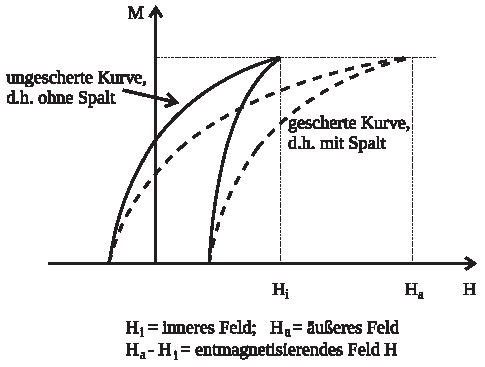
\includegraphics{Hysteresekurve_Scherung.pdf}
\caption{gescherte Hysteresekurve}
\end{figure}

In einem Ringkern ohne Luftspalt entspricht die Stärke des äußeren
Magnetfeldes \(H\) der des inneren Magnetfeldes \(H_E\). Mit einem
Luftspalt steigt \(H\) an, somit wird die Hystereseschleife nach außen
geschert. Daher lässt sich \(H_\mathrm{ent}\) durch die Scherung der
Hystereseschleife bestimmen.

\[
\begin{eqnarray}
    H_\mathrm{ent} &=& H - H_E \label{Hscher}
\end{eqnarray}
\]

\hypertarget{scheinbare-suszeptibilituxe4t}{%
\subsubsection{scheinbare
Suszeptibilität}\label{scheinbare-suszeptibilituxe4t}}

Bei konstanter Magnetisierung \(M\) kann die Suszeptibilität \(\chi\)
als Quotient \(\chi = \frac{M}{H}\) beschrieben werden, wobei \(H\) der
Betrag der Feldstärke zur Sättigungsmagnetisierung \(M\) ist.

Falls ein Luftspalt im Medium vorliegt, müssen die effektive Feldstärke
\(H_E\) im Kern und die Feldstärke \(H_L\) um Luftspalt betrachtet
werden. Daher gibt es eine \emph{scheinbare Suszeptibilität}
\(\chi_\mathrm{Schein}\) und eine \emph{wahre Suszeptibilität}
\(\chi_\mathrm{wahr}\). Nur die wahre Suszeptibilität
\(\chi_\mathrm{wahr}\) wirkt auf das effektiv wirkende Feld \(H_E\).

\[
\begin{eqnarray}
    \chi_\mathrm{Schein} &=& \frac{M}{H} \\
    \chi_\mathrm{wahr} &=& \frac{M}{H_E}
\end{eqnarray}
\]

Mit diesen Relationen kann man die wahre Suszeptibilität ermitteln.

\[
\begin{eqnarray}
    \eqref{defN} \Leftrightarrow H_\mathrm{ext} &=& NM
        \nonumber \\
        &=& HN\chi_\mathrm{Schein}
        \nonumber \\
    \eqref{Hscher} \Leftrightarrow H_E &=& H - H_\mathrm{ext}
        \nonumber \\
        &=& H - HN\chi_\mathrm{Schein}
        \nonumber \\
    \chi_\mathrm{wahr}
        &=& \frac{\chi_\mathrm{Schein} H}{H_E}
        \nonumber \\
        &=& \frac{\chi_\mathrm{Schein} H}{H - H_\mathrm{text}}
        \nonumber \\
        &=& \frac{\chi_\mathrm{Schein} H}{H - HN\chi_\mathrm{Schein}}
        \nonumber \\
    \chi_\mathrm{wahr}
        &=& \frac{\chi_\mathrm{Schein}}{1 - N\cdot\chi_\mathrm{Schein}} \label{ChiWahr}
\end{eqnarray}
\]

\hypertarget{durchfuxfchrung}{%
\section{Durchführung}\label{durchfuxfchrung}}

\hypertarget{versuchsaufbau}{%
\subsection{Versuchsaufbau}\label{versuchsaufbau}}

\begin{figure}
\centering
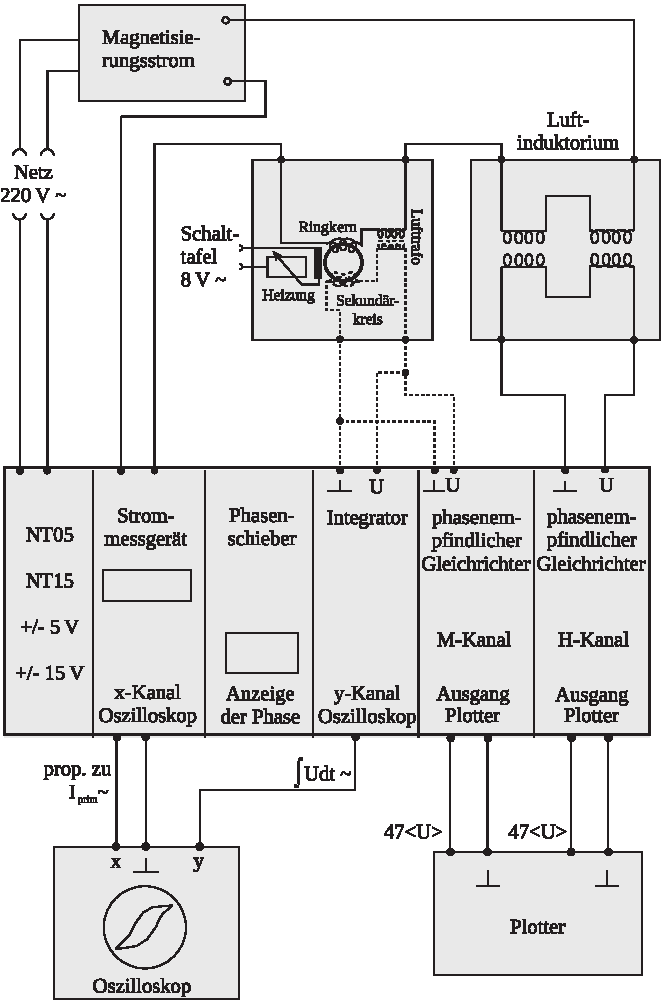
\includegraphics{Aufbau.pdf}
\caption{Versuchsaufbau}
\end{figure}

\hypertarget{messung-am-beheizbaren-ringkern}{%
\subsection{Messung am beheizbaren
Ringkern}\label{messung-am-beheizbaren-ringkern}}

\hypertarget{kenngruxf6uxdfenbestimmung}{%
\subsubsection{Kenngrößenbestimmung}\label{kenngruxf6uxdfenbestimmung}}

\hypertarget{kommutierungskurve}{%
\subsubsection{Kommutierungskurve}\label{kommutierungskurve}}

\hypertarget{suszeptibilituxe4t}{%
\paragraph{Suszeptibilität}\label{suszeptibilituxe4t}}

\hypertarget{temperaturabhuxe4ngigkeit-der-magnetisierung}{%
\subsubsection{Temperaturabhängigkeit der
Magnetisierung}\label{temperaturabhuxe4ngigkeit-der-magnetisierung}}

Am Phasenübergang ändert sich die Abhängigkeit qualitativ. Daher liegt
die Curie-Temperatur an der Stelle, an der die Messkurve einen Knick
hat. \#\# Messung am Ringkern mit Spalt \#\#\# Kenngrößenbestimmung
\#\#\# Entmagnetisierungsfaktor

\hypertarget{auswertung}{%
\section{Auswertung}\label{auswertung}}

\hypertarget{fazit}{%
\section{Fazit}\label{fazit}}

\hypertarget{literaturverzeichnis}{%
\section{Literaturverzeichnis}\label{literaturverzeichnis}}

\begin{enumerate}
\def\labelenumi{\arabic{enumi}.}
\tightlist
\item
  C. Kittel, Einführung in die Festkörperphysik, München: Oldenbourg
  Verlag, 2005
\item
  J. D. Jackson, Classical Elektrodynamics, New York: John Wiley \& Sons
  , 1962
\item
  E. Kneller, Ferromagnetismus, Berlin Heidelberg: Springer Verlag, 1962
\item
  W. Reith, Bergmann-Schaefer. Lehrbuch der Experimentalphysik.
  Elektromagnetismus, Bd. 2, Berlin: Walter de Gruyter Verlag, 2006
\item
  S. Hunklinger, Festkörperphysik, München: Oldenbourg Verlag, 2011
\item
  R. Gross und A. Marx, Festkörperphysik, München: Oldenbourg Verlag,
  2012
\item
  M. Fink, R.-D. Heuer und H. Kleinpoppen, Bergmann-Schaefer.
  Bestandteile der Materie, Bd. 4, W. Raith, Hrsg., Berlin: Walter de
  Gruyter Verlag, 2003
\item
  Universität zu Köln, ``Anleitung zum Versuch 2.4 Magnetisierung eines
  Ferrits'', Juni 2013, Online verfügbar unter
  \url{http://www.ph2.uni-koeln.de/fileadmin/Lehre/PraktikumB/B2.4.pdf}
\end{enumerate}

\end{document}
